\documentclass[11pt,a4paper]{article}

\usepackage[margin=2.5cm]{geometry}
\usepackage{amsmath}
\usepackage{booktabs}
\usepackage{hyperref}
\usepackage{url}
\usepackage{xcolor}
\usepackage{graphicx}
\usepackage{pgfplots}
\pgfplotsset{compat=1.18}
\usepackage{caption}
\usepackage{subcaption}
\usepackage{parskip}
\usepackage{microtype}
\usepackage{titlesec}

\titlespacing*{\section}{0pt}{12pt}{6pt}
\titlespacing*{\subsection}{0pt}{8pt}{4pt}

\hypersetup{colorlinks=true, linkcolor=blue, citecolor=blue, urlcolor=blue}

\title{\textbf{Continual Fine-Tuning of Small Language Models}\\
\large Comparing Anti-Forgetting Strategies on Sequential ArXiv Batches}
\author{Benny Lay}
\date{May 2026}

\begin{document}

\maketitle

\begin{abstract}
When a language model is fine-tuned sequentially on multiple datasets, it tends to forget what it learned earlier, a well-known problem called catastrophic forgetting. This project compares five strategies to limit this effect on Qwen2-0.5B, trained on quarterly batches of ArXiv abstracts (2024): naive fine-tuning, EWC with and without Fisher accumulation, LoRA with experience replay, and Orthogonal LoRA (O-LoRA). The LoRA-based methods work well; EWC does not, at least in this intra-domain setting. The most interesting result is that O-LoRA, which never stores old data, performs almost identically to LoRA+Replay, making it a practical option when data retention is not possible.
\end{abstract}

\section{Introduction}

A language model trained on last year's data will eventually be out of date. 
The natural solution is to keep fine-tuning it as new data arrives. 
The problem is that this tends to destroy what the model already knew. 
Indeed, each new training step shifts the weights toward the new data, overwriting older knowledge. 
This is called \textit{catastrophic forgetting}.

This project was built to get hands-on experience with the main strategies used to address this problem, in the context of small language models. 
Qwen2-0.5B (500M parameters) was fine-tuned on four quarterly batches of ArXiv abstracts from 2024, covering machine learning (cs.LG) and natural language processing (cs.CL). 
After each batch, perplexity on all previous batches was measured to track how much the model forgets. Five training strategies are compared.

\section{Methods}

\subsection{Data}

Each batch contains 500 abstracts fetched from the ArXiv API, from papers published in a given quarter of 2024 (cs.LG and cs.CL). Abstracts are tokenized with Qwen2's BPE tokenizer, truncated to 512 tokens, and padded to a fixed length. The four batches are processed one after the other, without any shuffling across quarters.

\subsection{Model}

Qwen2-0.5B\footnote{\url{https://huggingface.co/Qwen/Qwen2-0.5B}} is a 500M parameter causal language model. 
The choice was motivated by its size: small enough to train on a single GPU (e.g. NVIDIA RTX 5080), while still being a real model with competitive base performance. 
All experiments run in bfloat16 precision.

\subsection{Training Strategies}

\paragraph{Naive.} \mbox{}\\

Standard full-weight fine-tuning with no forgetting protection. 
It serves as the baseline.

\paragraph{EWC ($\lambda$=0.4).} \mbox{}\\

Elastic Weight Consolidation \cite{kirkpatrick2017overcoming} adds a regularization term penalizing changes to parameters that were important for previous tasks, as measured by the diagonal Fisher information matrix:
\[
\mathcal{L}_{\text{total}} = \mathcal{L}_{\text{task}} + \frac{\lambda}{2} \sum_i F_i \cdot (\theta_i - \theta_i^*)^2
\]
Here, the Fisher matrix is recomputed and replaced at each step ($\lambda = 0.4$).

\paragraph{EWC accumulated ($\lambda$=5.0).} \mbox{}\\

Same as above, but the Fisher matrix is \textit{accumulated} across all seen batches ($F_{\text{total}} = F_1 + F_2 + \ldots$) and a stronger regularization coefficient is used ($\lambda = 5.0$). This addresses a known limitation of single-step EWC.

\paragraph{LoRA + Replay.} \mbox{}\\

Low-Rank Adaptation \cite{hu2022lora} restricts weight updates to low-rank increments $\Delta W = AB$ (rank $r=8$, only 0.11\% of parameters are trained). After training on each new batch, 20\% of the training data is sampled from all previous batches (\textit{experience replay}) and mixed with the current batch data. After each batch, adapters are merged into the base weights and re-initialized.

\paragraph{O-LoRA.} \mbox{}\\

Orthogonal LoRA adds a penalty discouraging the new batch's adapter subspace from overlapping with those of previous batches:
\[
\mathcal{L}_{\text{orth}} = \lambda_{\text{orth}} \sum_{\ell} \| A_{\ell}^{(t)} \cdot (A_{\ell}^{(t-1)})^\top \|_F^2
\]
where $A_{\ell}^{(t)}$ is the LoRA $A$ matrix at layer $\ell$ after training on batch $t$. This encourages each batch to learn in a distinct subspace, preventing new learning from overwriting old representations, all without storing any past data ($\lambda_{\text{orth}} = 1.0$).

\section{Results}

\subsection{Perplexity and Catastrophic Forgetting}

Table~\ref{tab:ppl_b01} shows how perplexity on batch\_01 evolves as the model trains on later batches. A rising perplexity means the model is forgetting.

\begin{table}[h]
\centering
\caption{Perplexity on batch\_01 after sequential training (lower = less forgetting).}
\label{tab:ppl_b01}
\begin{tabular}{lcccc}
\toprule
\textbf{Strategy} & \textbf{After B01} & \textbf{After B02} & \textbf{After B03} & \textbf{After B04} \\
\midrule
Naive                      & 2.55 & 4.12 & 4.82 & 5.14 \\
EWC ($\lambda$=0.4)        & 2.61 & 3.72 & 4.69 & 5.02 \\
EWC accumulated ($\lambda$=5.0) & 2.60 & 3.73 & 4.64 & 5.05 \\
LoRA + Replay              & 3.83 & 3.68 & 3.67 & \textbf{3.66} \\
O-LoRA                     & 3.83 & 3.71 & 3.70 & \textbf{3.70} \\
\bottomrule
\end{tabular}
\end{table}

\begin{figure}[h]
\centering
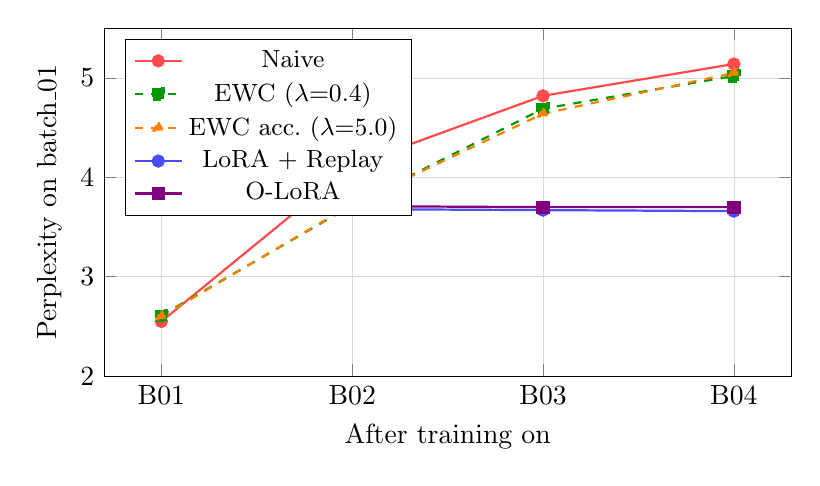
\begin{tikzpicture}
\begin{axis}[
    width=0.85\textwidth,
    height=6cm,
    xlabel={After training on},
    ylabel={Perplexity on batch\_01},
    xtick={1,2,3,4},
    xticklabels={B01,B02,B03,B04},
    legend pos=north west,
    legend style={font=\small},
    grid=both,
    grid style={line width=0.2pt, draw=gray!30},
    ymin=2, ymax=5.5,
]
\addplot[color=red!70,   mark=*, thick] coordinates {(1,2.55)(2,4.12)(3,4.82)(4,5.14)};
\addplot[color=green!60!black, mark=square*, thick, dashed] coordinates {(1,2.61)(2,3.72)(3,4.69)(4,5.02)};
\addplot[color=orange,   mark=triangle*, thick, dashed] coordinates {(1,2.60)(2,3.73)(3,4.64)(4,5.05)};
\addplot[color=blue!70,  mark=*, thick] coordinates {(1,3.83)(2,3.68)(3,3.67)(4,3.66)};
\addplot[color=violet,   mark=square*, thick] coordinates {(1,3.83)(2,3.71)(3,3.70)(4,3.70)};
\legend{Naive, EWC ($\lambda$=0.4), EWC acc.\ ($\lambda$=5.0), LoRA + Replay, O-LoRA}
\end{axis}
\end{tikzpicture}
\caption{Perplexity on batch\_01 across training steps. LoRA-based methods remain stable; EWC and Naive degrade significantly.}
\label{fig:ppl_curve}
\end{figure}

Table~\ref{tab:forgetting} puts a number on the total forgetting: how much has perplexity on batch\_01 changed between the moment we first trained on it and the end of the full sequence.

\begin{table}[h]
\centering
\caption{Catastrophic forgetting summary on batch\_01 (B01 → B04).}
\label{tab:forgetting}
\begin{tabular}{lccc}
\toprule
\textbf{Strategy} & \textbf{PPL after B01} & \textbf{PPL after B04} & \textbf{Forgetting} \\
\midrule
Naive                      & 2.55 & 5.14 & $+$101.6\% \\
EWC ($\lambda$=0.4)        & 2.61 & 5.02 & $+$92.3\%  \\
EWC accumulated ($\lambda$=5.0) & 2.60 & 5.05 & $+$94.2\% \\
LoRA + Replay              & 3.83 & \textbf{3.66} & $-$4.4\% \\
O-LoRA                     & 3.83 & \textbf{3.70} & $-$3.4\% \\
\bottomrule
\end{tabular}
\end{table}

LoRA + Replay and O-LoRA are the only strategies that actually work. Interestingly, both \textit{improve} slightly on batch\_01 as training continues: the model gets better at it even without seeing it again directly. Their starting perplexity after B01 (3.83) is higher than Naive (2.55) because LoRA constrains the update space and takes a bit more time to converge.

\subsection{Benchmark Evaluation}

The LoRA + Replay checkpoints were also evaluated on three standard zero-shot benchmarks using the LM Evaluation Harness \cite{lmeval}: ARC-Easy \cite{arc} (factual science questions), HellaSwag \cite{hellaswag} (commonsense reasoning), and PIQA \cite{piqa} (physical intuition).

\begin{table}[h]
\centering
\caption{Zero-shot benchmark accuracy (\%) across LoRA+Replay training stages.}
\label{tab:benchmarks}
\begin{tabular}{lccccc}
\toprule
\textbf{Task} & \textbf{Base} & \textbf{After B01} & \textbf{After B02} & \textbf{After B03} & \textbf{After B04} \\
\midrule
ARC-Easy  & 54.84 & 56.52 & 57.70 & 58.21 & 57.03 \\
HellaSwag & 38.39 & 38.10 & 38.12 & 37.95 & 38.08 \\
PIQA      & 69.37 & 69.04 & 67.52 & 68.23 & 68.23 \\
\bottomrule
\end{tabular}
\end{table}

ARC-Easy improves by about 2\% after B03, which makes sense: the model is reading ML and NLP papers, and ARC tests the kind of factual knowledge that comes up in those texts. HellaSwag barely moves, and PIQA drops by about 1\%. Physical intuition is not something you pick up from reading abstracts about transformer architectures.

\section{Discussion}

\paragraph{Why does EWC fail?} \mbox{}\\
EWC uses the Fisher matrix to find which parameters matter most for past tasks, then penalizes changes to them. The issue here is that all four batches come from the same domain: ML and NLP papers from 2024. Because the data is so similar, the gradients look alike across batches, and the Fisher matrix cannot tell apart "important for batch\_01'' from "important for batch\_04''. The penalty ends up spread across the same parameters every time, which is too diffuse to actually protect anything. Accumulating Fisher ($\lambda=5.0$) does not fix this: the signal was never there to begin with.

\paragraph{Why does O-LoRA match LoRA + Replay?} \mbox{}\\
Both methods ultimately do the same thing: they prevent new training from overwriting old representations. They just go about it differently.
\begin{itemize}
    \item LoRA + Replay keeps 20\% of old data in each training step, so the model is explicitly forced to stay good on past batches.
    \item O-LoRA pushes each new batch's adapter subspace to be orthogonal to the previous one, so the new update physically cannot land in the same direction as the old one.
\end{itemize}
The results are nearly identical (3.66 vs.\ 3.70). For this domain, structural separation through geometry is just as effective as structural separation through data. O-LoRA needs no stored data, only the previous $A$ matrices, which cost essentially nothing.

\paragraph{Limitations.}\mbox{}\\
This is a single model, a single domain, and a small number of batches. Whether these conclusions hold for more diverse task sequences, or for larger models where LoRA covers a smaller fraction of the total capacity, is an open question. Perplexity also only measures how surprised the model is by text, not how well it performs on actual tasks. Running O-LoRA through the same benchmarks as LoRA + Replay would be a useful next step.

\section{Conclusion}

EWC, despite its theoretical appeal, does not work well when training batches come from the same domain. 
LoRA-based methods do, and the gap is large. The most useful takeaway is that O-LoRA achieves nearly the same result as LoRA + Replay, without keeping any old data. 
In practice, this matters whenever storing past training data is expensive, restricted, or simply not an option.

Several directions are worth exploring: testing on more heterogeneous task sequences, training for more than one epoch per batch, running downstream benchmarks on O-LoRA checkpoints, and combining O-LoRA with a small replay buffer.

\begin{thebibliography}{9}

\bibitem{kirkpatrick2017overcoming}
J.\ Kirkpatrick et al., "Overcoming catastrophic forgetting in neural networks,'' \textit{PNAS}, 2017.
\url{https://doi.org/10.1073/pnas.1611835114}

\bibitem{hu2022lora}
E.\ J.\ Hu et al., "LoRA: Low-Rank Adaptation of Large Language Models,'' \textit{ICLR}, 2022.
\url{https://doi.org/10.48550/arXiv.2106.09685}

\bibitem{lmeval}
L.\ Gao et al., "A Framework for Few-Shot Language Model Evaluation,'' \textit{Zenodo}, 2021.

\bibitem{arc}
P.\ Clark et al., "Think you have Solved Question Answering? Try ARC,'' 2018.
\url{https://doi.org/10.48550/arXiv.1803.05457}

\bibitem{hellaswag}
R.\ Zellers et al., "HellaSwag: Can a Machine Really Finish Your Sentence?,'' \textit{ACL}, 2019.
\url{https://doi.org/10.48550/arXiv.1905.07830}

\bibitem{piqa}
Y.\ Bisk et al., "PIQA: Reasoning about Physical Commonsense in Natural Language,'' \textit{AAAI}, 2020.
\url{https://doi.org/10.48550/arXiv.1911.11641}
\end{thebibliography}

\end{document}
